
\documentclass{article}
\usepackage[utf8]{inputenc}
\usepackage{graphicx}
\usepackage{float}

\begin{document}

\begin{figure}[H]
\centering
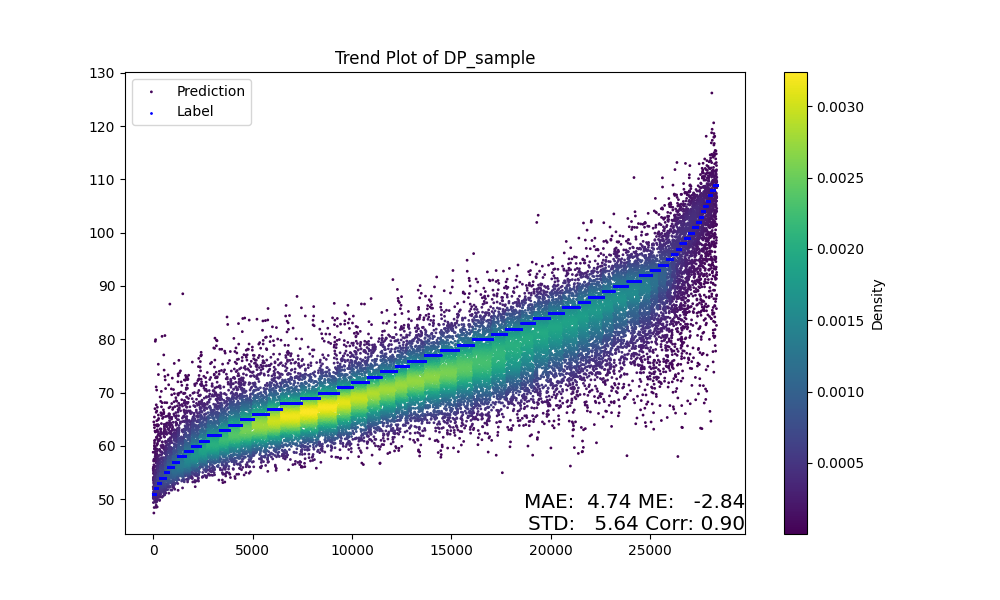
\includegraphics[width=\textwidth]{./Fig/Trend_Plot_DP_sample.png}
\caption{Trend Plot}
\label{fig:image1}
\end{figure}

\begin{figure}[H]
\centering
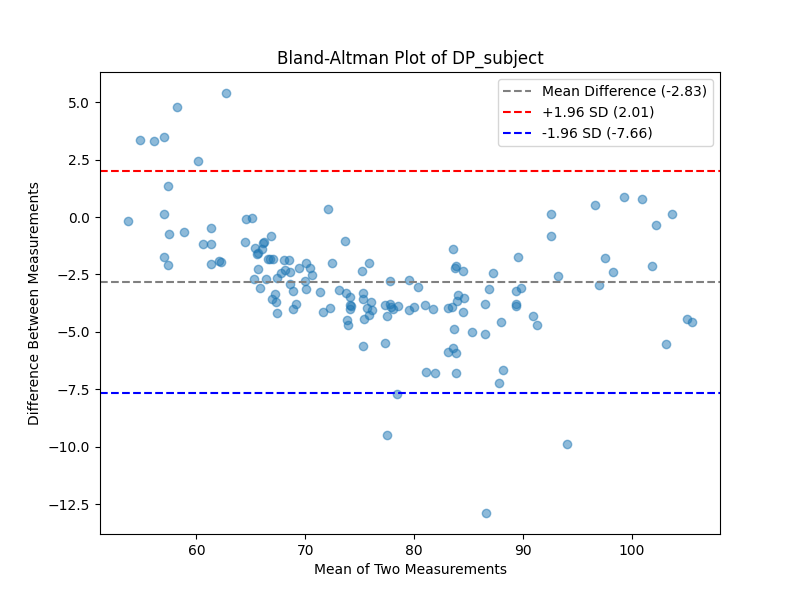
\includegraphics[width=0.8\textwidth]{./Fig/Bland_Altman_Plot_DP_subject.png}
\caption{Bland Altman Plot of subject level}
\label{fig:image2}
\end{figure}

\begin{figure}[H]
\centering
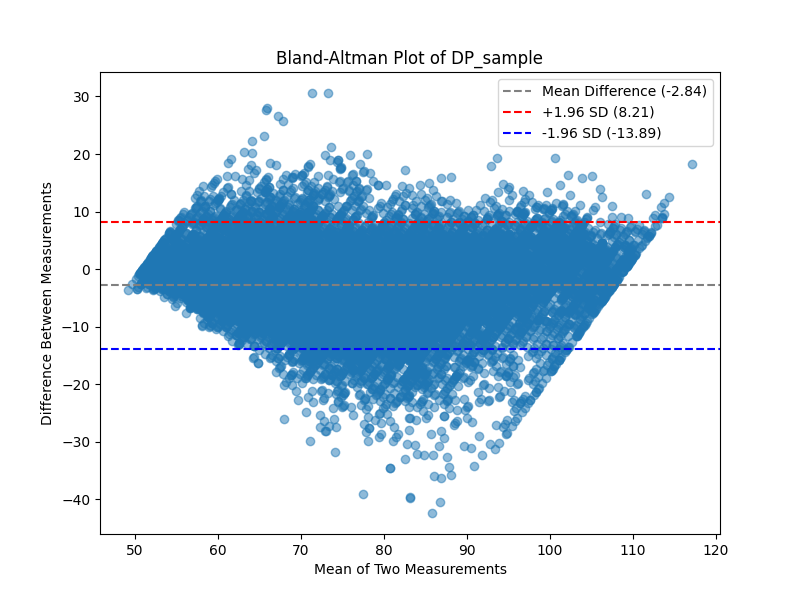
\includegraphics[width=0.8\textwidth]{./Fig/Bland_Altman_Plot_DP_sample.png}
\caption{Bland Altman Plot of sample level}
\label{fig:image2}
\end{figure}

\begin{figure}[H]
\centering
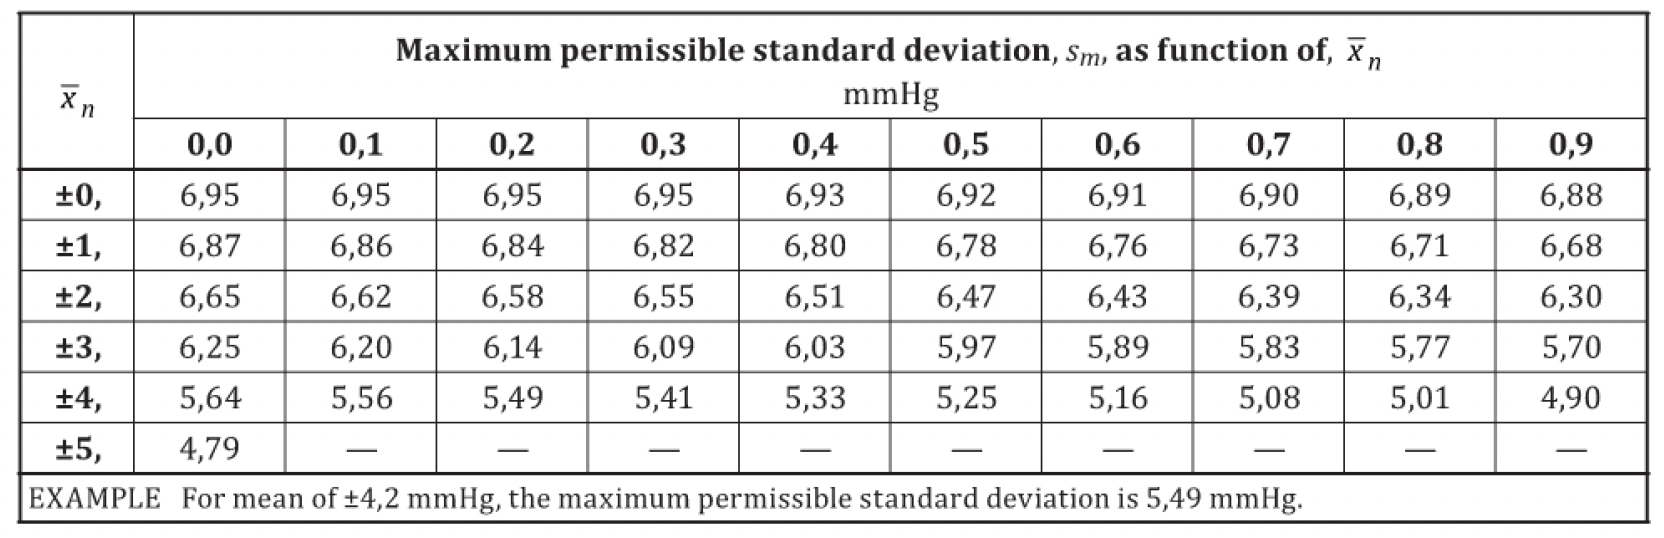
\includegraphics[width=0.8\textwidth]{./Fig/ME_STD_Correspond.png}
\caption{Averaged subject data acceptance in mmHg}
\label{ME_STD}
\end{figure}

\begin{table}[h!]
\centering
\begin{tabular}{|c|c|c|c|c|}
\hline
Level & ME & MAE & SD & Correlation \\ \hline
Sample Level & -2.84 & 4.74 & 5.64 & 0.90 \\ \hline
Subject Level & -2.83 & 3.20 & 2.47 & 0.98 \\ \hline
\end{tabular}
\caption{Prediction Results}
\label{tab:metrics}
\end{table}

\end{document}
